\documentclass{beamer}
\usepackage[utf8]{inputenc}
\usepackage[export]{adjustbox}
\usepackage{hyperref}
\hypersetup{
	colorlinks=true,
	urlcolor=adcorange,
	linkcolor=adcblue
}

\usetheme{Madrid}

\title{Let's make a todo list app with React Native!}
\subtitle{AsyncStorage!}
\author{Nathaniel Budijono}
\date{February 15, 2022}
\institute{UMN ADC}

\definecolor{adcblue}{RGB}{115,203,255}
\definecolor{adcorange}{RGB}{242,114,0}

\setbeamercolor{palette primary}{fg=white,bg=adcblue}
\setbeamercolor{palette secondary}{fg=adcorange,bg=white}
\setbeamercolor{structure}{fg=adcblue,bg=white}
\setbeamercolor{title in head/foot}{fg=adcblue,bg=white}
\setbeamercolor{date in head/foot}{fg=gray,bg=white}
\setbeamercolor{palette tertiary}{fg=white,bg=adcorange}

\begin{document}

\begin{frame}
    \titlepage
    \includegraphics[width=0.25\textwidth, right]{figs/ADC_Logo_Blue.png}
\end{frame}

\begin{frame}{Officer openings!}
	\begin{itemize}
		\item Workshop instructors
	\end{itemize}

	\bigskip

	DM us on the discord!

	\bigskip

	\href{https://z.umn.edu/ADCdiscord}{https://z.umn.edu/ADCdiscord}
\end{frame}

\begin{frame}{Guide}
	We will be following this guide: \href{https://github.com/ADC-UMN/todotorial}{https://github.com/ADC-UMN/todotorial}. Feel free to go ahead of the workshops at your own pace.
\end{frame}

\begin{frame}{What we're starting with}
	\centering
	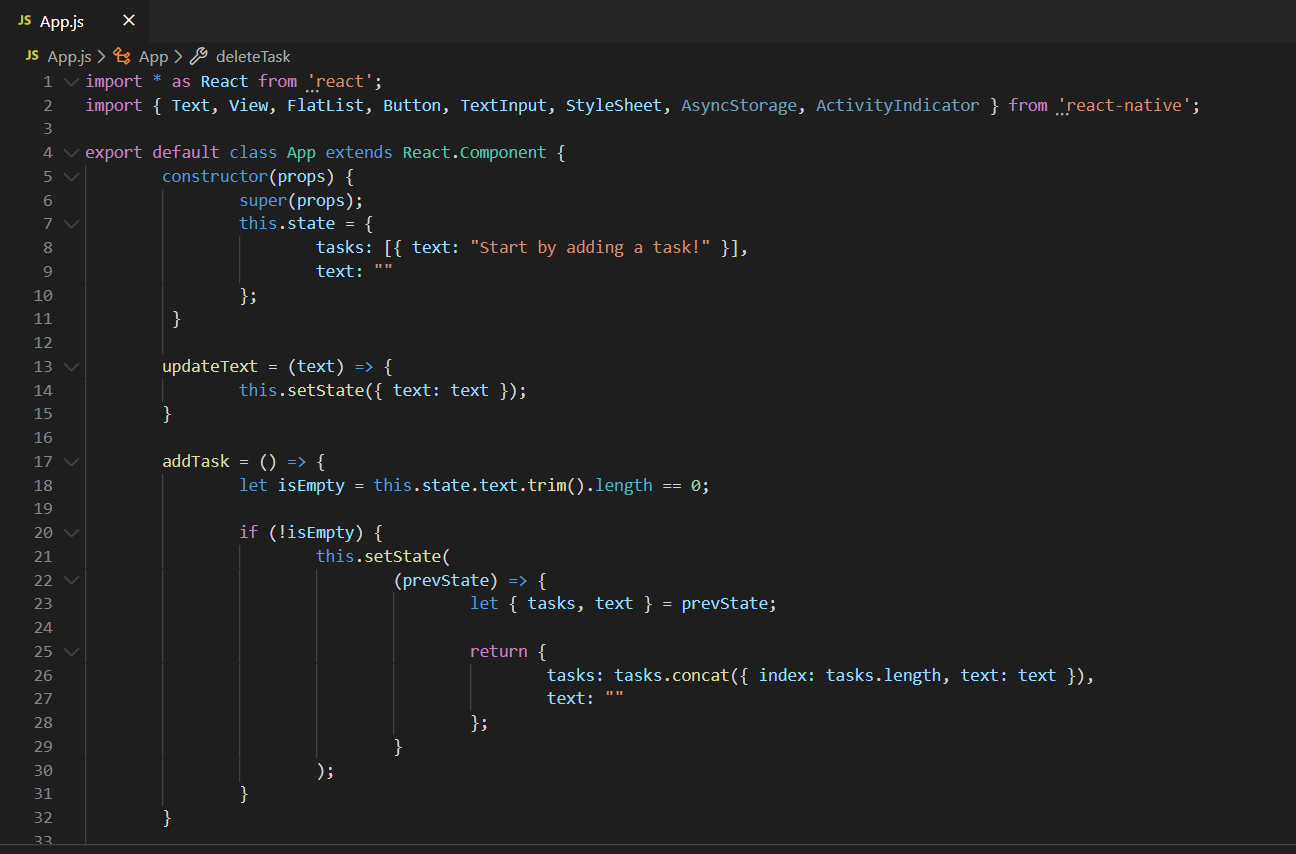
\includegraphics[width=0.9\textwidth]{figs/after-state.png}	
\end{frame}

\begin{frame}{Goals}
	\begin{enumerate}
		\item Ability to have the state of the app persist between sessions
	\end{enumerate}
\end{frame}

\begin{frame}{Research}
	\begin{itemize}
		\item Default React Native AsyncStorage \href{https://reactnative.dev/docs/asyncstorage}{https://reactnative.dev/docs/asyncstorage} \pause
		\begin{itemize}
			\item Deprecated \pause
		\end{itemize}
		\item Use a community package instead \href{https://react-native-async-storage.github.io/async-storage/}{https://react-native-async-storage.github.io/async-storage/}
	\end{itemize}
\end{frame}

\begin{frame}{What is Async?}
	Asynchronous

	\bigskip\pause

	Callbacks, Promises, Async/Await

	\bigskip

	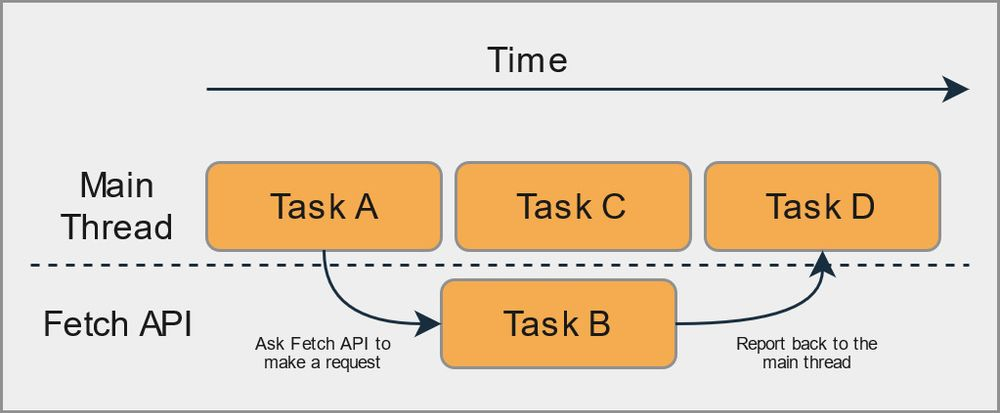
\includegraphics[width=0.9\textwidth]{figs/asynchronous.jpg}
\end{frame}

\begin{frame}{Read from AsyncStorage}
	\begin{enumerate}
		\item Write a \texttt{componentDidMount()} \pause
		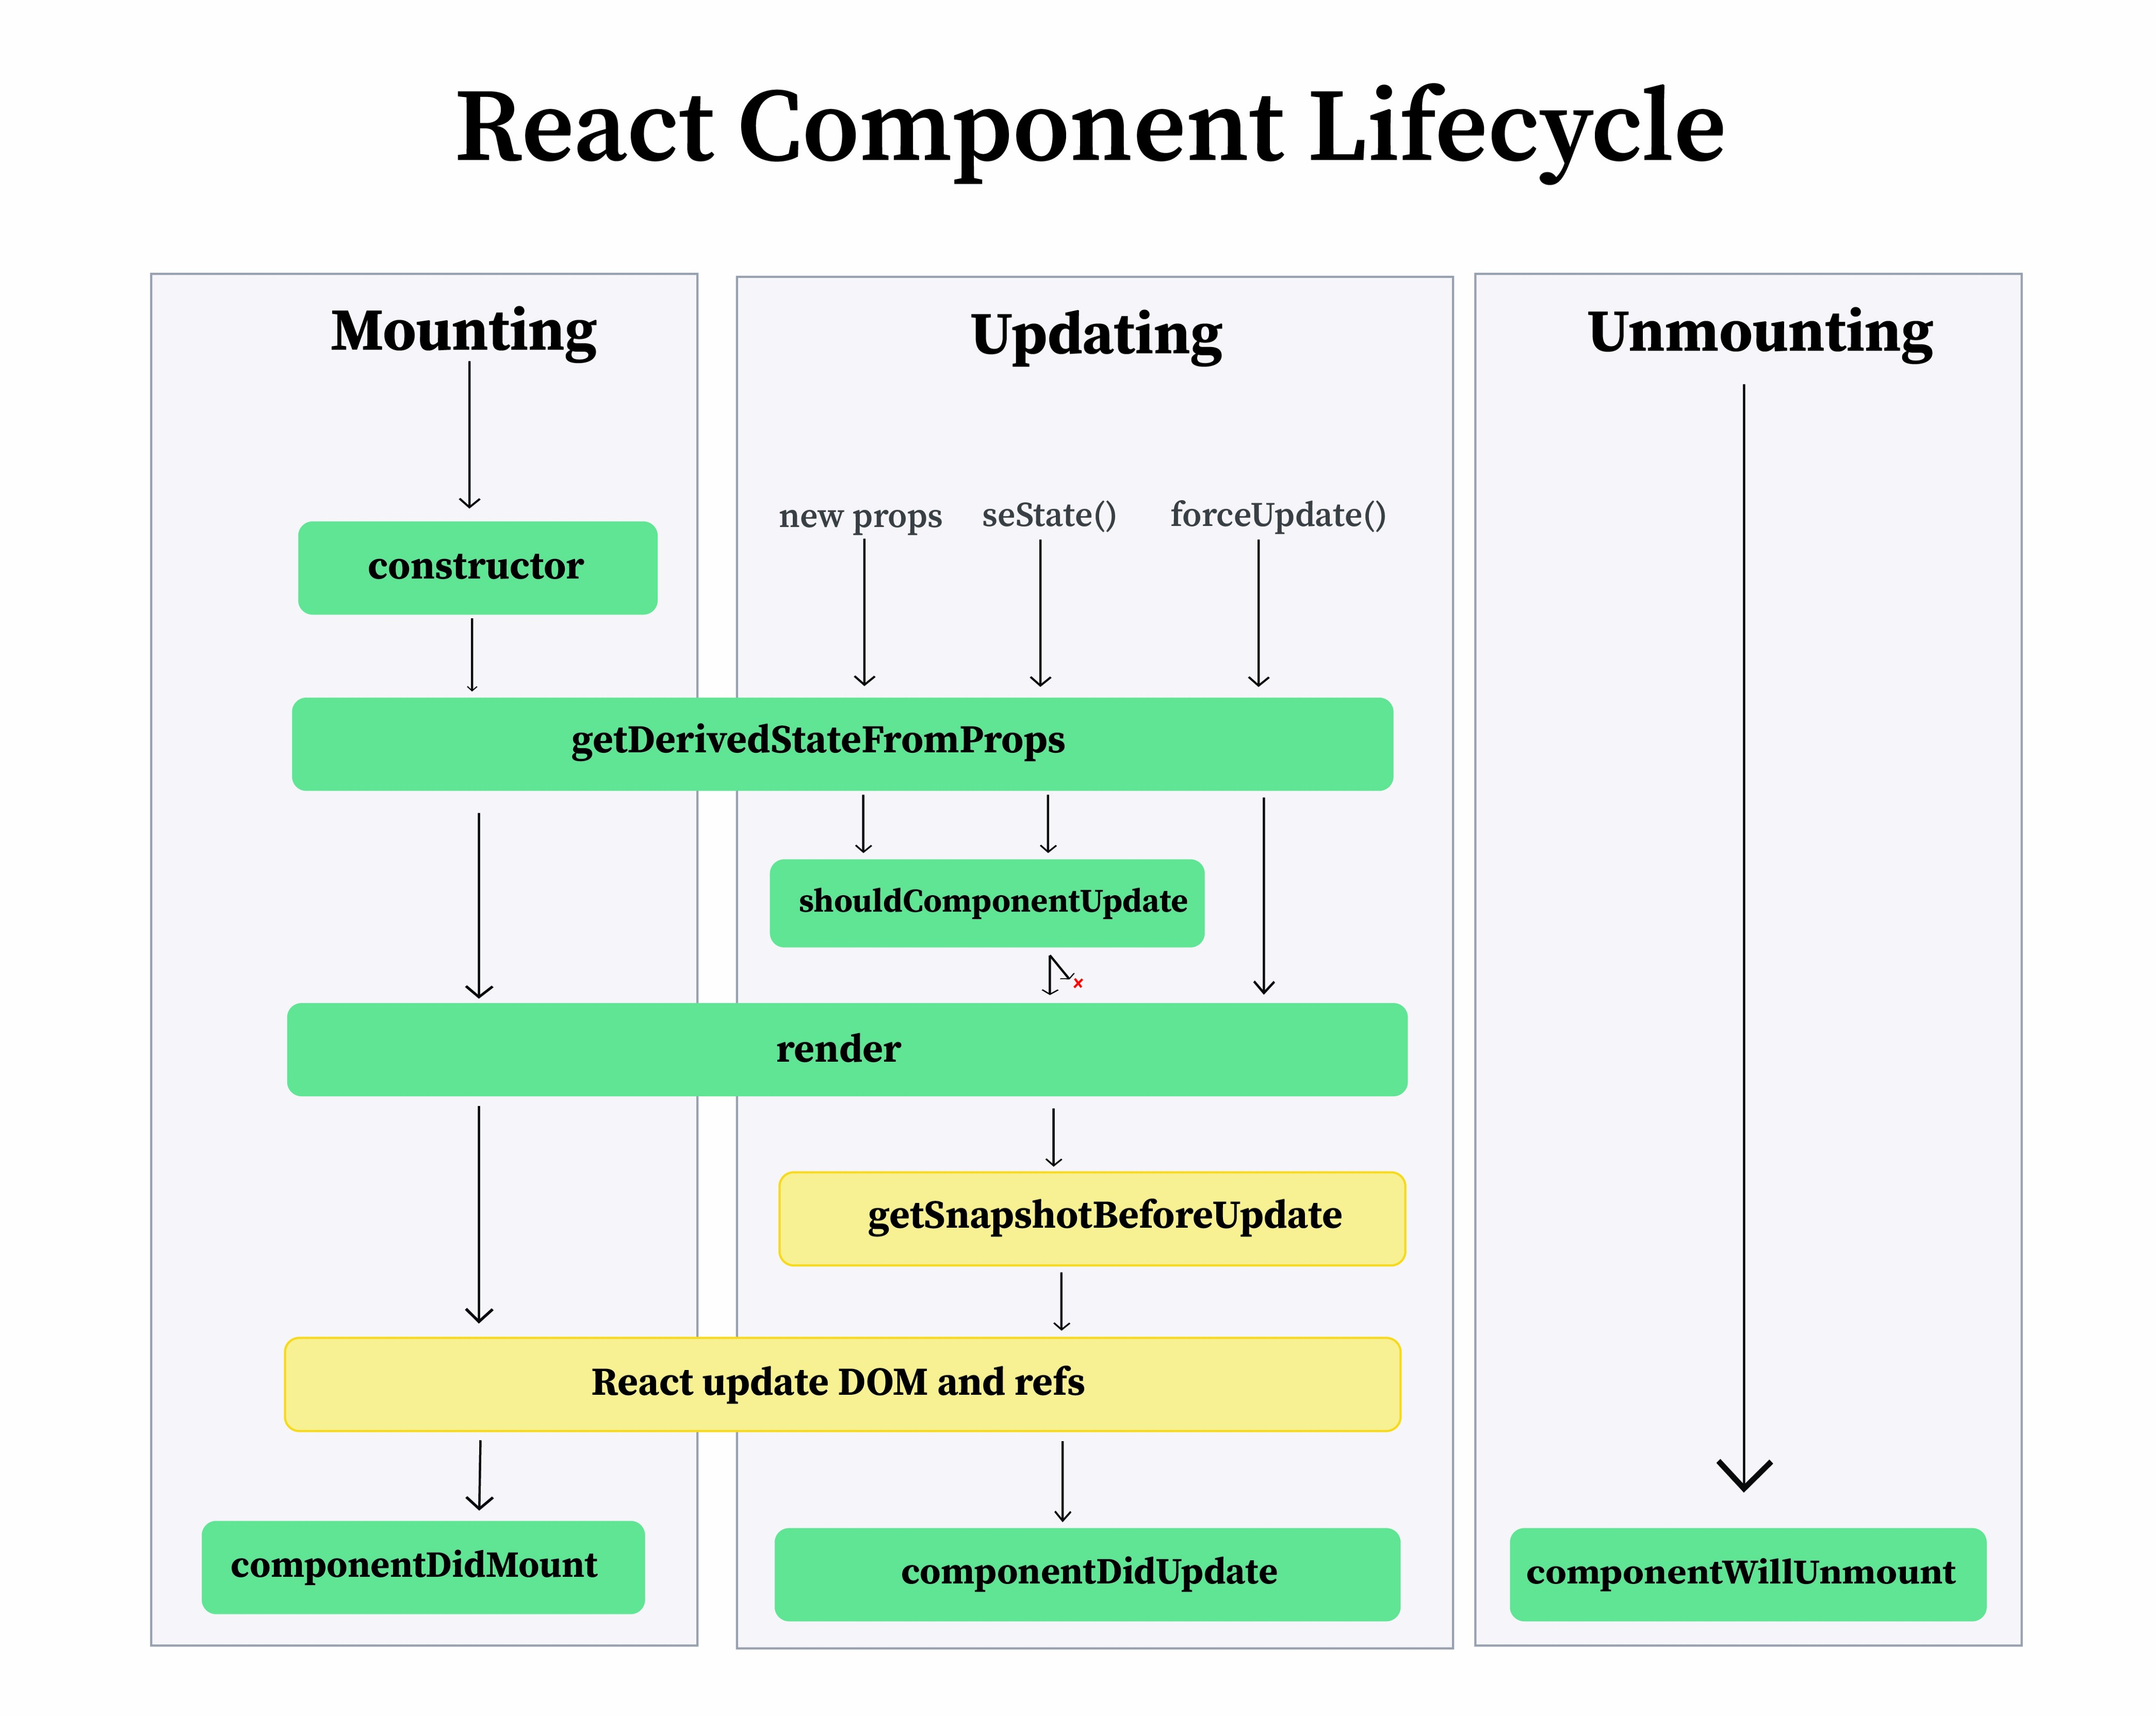
\includegraphics[width=0.8\textwidth]{figs/component-lifecycle.jpeg}
	\end{enumerate}
\end{frame}

\begin{frame}{Write to AsyncStorage}
	\begin{enumerate}
		\item Modify \texttt{addTask()} \pause
		\item Modify \texttt{deleteTask()}
	\end{enumerate}
\end{frame}

\end{document}